%%%%%%%%%%%%%%%%%%%%%%%%%%%%%%%%%%%%%%%%%
% Masters/Doctoral Thesis 
% LaTeX Template
% Version 2.5 (27/8/17)
%
% This template was downloaded from:
% http://www.LaTeXTemplates.com
%
% Version 2.x major modifications by:
% Vel (vel@latextemplates.com)
%
% This template is based on a template by:
% Steve Gunn (http://users.ecs.soton.ac.uk/srg/softwaretools/document/templates/)
% Sunil Patel (http://www.sunilpatel.co.uk/thesis-template/)
%
% Template license:
% CC BY-NC-SA 3.0 (http://creativecommons.org/licenses/by-nc-sa/3.0/)
%
%%%%%%%%%%%%%%%%%%%%%%%%%%%%%%%%%%%%%%%%%

%----------------------------------------------------------------------------------------
%	PACKAGES AND OTHER DOCUMENT CONFIGURATIONS
%----------------------------------------------------------------------------------------
\documentclass[
11pt, % The default document font size, options: 10pt, 11pt, 12pt
oneside, % Two side (alternating margins) for binding by default, uncomment to switch to one side
english, % ngerman for German
singlespacing, % Single line spacing, alternatives: onehalfspacing or doublespacing
%draft, % Uncomment to enable draft mode (no pictures, no links, overfull hboxes indicated)
%nolistspacing, % If the document is onehalfspacing or doublespacing, uncomment this to set spacing in lists to single
%liststotoc, % Uncomment to add the list of figures/tables/etc to the table of contents
%toctotoc, % Uncomment to add the main table of contents to the table of contents
%parskip, % Uncomment to add space between paragraphs
%nohyperref, % Uncomment to not load the hyperref package
headsepline, % Uncomment to get a line under the header
chapterinoneline, % Uncomment to place the chapter title next to the number on one line
%consistentlayout, % Uncomment to change the layout of the declaration, abstract and acknowledgements pages to match the default layout
]{MastersDoctoralThesis} % The class file specifying the document structure

\usepackage[utf8]{inputenc} % Required for inputting international characters
\usepackage[T1]{fontenc} % Output font encoding for international characters
\usepackage{mathpazo} % Use the Palatino font by default
\usepackage{cite}

%\usepackage[backend=bibtex,style=numeric,sorting=none, maxbibnames=99]{biblatex} % Use the bibtex backend with the authoryear citation style (which resembles APA)

%\addbibresource{~/BibTex/BibTex.bib} % The filename of the bibliography

\usepackage[autostyle=true]{csquotes} % Required to generate language-dependent quotes in the bibliography

\usepackage{amstext, amsfonts, amsmath, amsbsy, amssymb}
\usepackage{tikz}
\usepackage{booktabs}
\usepackage{pgfplots}

%----------------------------------------------------------------------------------------
%	MARGIN SETTINGS
%----------------------------------------------------------------------------------------

\geometry{
	paper=a4paper, % Change to letterpaper for US letter
	inner=2.5cm, % Inner margin
	outer=3.8cm, % Outer margin
	bindingoffset=.5cm, % Binding offset
	top=1.5cm, % Top margin
	bottom=1.5cm, % Bottom margin
	%showframe, % Uncomment to show how the type block is set on the page
}

%----------------------------------------------------------------------------------------
%	THESIS INFORMATION
%----------------------------------------------------------------------------------------

\thesistitle{Anticipating the chemical compositions of organisms across the tree of life.} % Your thesis title, this is used in the title and abstract, print it elsewhere with \ttitle
\supervisor{Prof. Daniel \textsc{Wegmann} \\ \& Dr. Pierre-Marie \textsc{Allard}} % Your supervisor's name, this is used in the title page, print it elsewhere with \supname
\examiner{} % Your examiner's name, this is not currently used anywhere in the template, print it elsewhere with \examname
\degree{Master of Science in Bioinformatics and Computational Biology} % Your degree name, this is used in the title page and abstract, print it elsewhere with \degreename
\author{Marco \textsc{Visani}} % Your name, this is used in the title page and abstract, print it elsewhere with \authorname
\addresses{} % Your address, this is not currently used anywhere in the template, print it elsewhere with \addressname

\subject{Biological Sciences} % Your subject area, this is not currently used anywhere in the template, print it elsewhere with \subjectname
\keywords{} % Keywords for your thesis, this is not currently used anywhere in the template, print it elsewhere with \keywordnames
\university{\href{https://www.unifr.ch/}{University of Fribourg}} % Your university's name and URL, this is used in the title page and abstract, print it elsewhere with \univname
\department{\href{https://www.unifr.ch/bio/en/}{Department of Biology}} % Your department's name and URL, this is used in the title page and abstract, print it elsewhere with \deptname
\group{\href{https://www.unifr.ch/bio/en/groups/wegmann/}{Wegmann Group} \& \href{https://www.unifr.ch/bio/en/groups/allard/}{COMMONS Lab}} % Your research group's name and URL, this is used in the title page, print it elsewhere with \groupname
\faculty{\href{https://www.unifr.ch/scimed/en/}{Faculty of Science and Medicine}} % Your faculty's name and URL, this is used in the title page and abstract, print it elsewhere with \facname

\AtBeginDocument{
\hypersetup{pdftitle=\ttitle} % Set the PDF's title to your title
\hypersetup{pdfauthor=\authorname} % Set the PDF's author to your name
\hypersetup{pdfkeywords=\keywordnames} % Set the PDF's keywords to your keywords
}


%----------------------------------------------------------------------------------------
%	MATH STUFF
\usepackage{amstext, amsfonts, amsmath, amsbsy, amssymb}
\DeclareMathOperator{\Poisson}{Poisson}
\DeclareMathOperator{\Multinom}{Multinom}
\DeclareMathOperator{\logit}{logit}
\DeclareMathOperator{\cov}{cov}
\DeclareMathOperator{\Ind}{I}
\def\P{\mathbb{P}}
\def\E{\mathbb{E}}

\def\x{\boldsymbol{x}}

\def\btau{\boldsymbol{\tau}}
\def\bmu{\boldsymbol{\mu}}
\def\bxi{\boldsymbol{\xi}}
\def\bLambda{\boldsymbol{\Lambda}}
\def\bP{\boldsymbol{P}}
\def\bd{\boldsymbol{d}}


\def\Ccal{{\cal C}}
\def\E{{\cal E}}
\def\I{{\cal I}}
\def\N{{\cal N}}
\def\M{{\cal M}}
\def\R{{\cal R}}
\def\T{{\cal T}}
\def\X{{\cal X}}
\def\Y{{\cal Y}}
\def\Z{{\cal Z}}


%----------------------------------------------------------------------------------------

\linespread{1.25}
\begin{document}


\frontmatter % Use roman page numbering style (i, ii, iii, iv...) for the pre-content pages

\pagestyle{plain} % Default to the plain heading style until the thesis style is called for the body content

%----------------------------------------------------------------------------------------
%	TITLE PAGE
%----------------------------------------------------------------------------------------

\begin{titlepage}
\begin{center}

\vspace*{.06\textheight}
{\scshape\LARGE \univname\par}\vspace{1.5cm} % University name
\textsc{\Large Master Thesis}\\[0.5cm] % Thesis type

\HRule \\[0.4cm] % Horizontal line
{\huge \bfseries \ttitle\par}\vspace{0.4cm} % Thesis title
\HRule \\[1.5cm] % Horizontal line
 
\begin{minipage}[t]{0.4\textwidth}
\begin{flushleft} \large
\emph{Author:}\\
\href{mailto:contact@vismarco.ch}{\authorname} % Author name - remove the \href bracket to remove the link
\end{flushleft}
\end{minipage}
\begin{minipage}[t]{0.4\textwidth}
\begin{flushright} \large
\emph{Supervisors:} \\
\href{mailto:daniel.wegmann@unifr.ch}{Prof. Daniel \textsc{Wegmann}} \\
\href{mailto:pierre-marie.allard@unifr.ch}{Dr. Pierre-Marie \textsc{Allard}}% Supervisor name - remove the \href bracket to remove the link  
\end{flushright}
\end{minipage}\\[3cm]
 
\vfill

\large \textit{A thesis submitted in fulfillment of the requirements \\ for the degree of \degreename}\\[0.3cm] % University requirement text
\textit{in the}\\[0.4cm]
\groupname\\\deptname\\[2cm] % Research group name and department name
 
\vfill

{\large \today}\\[4cm] % Date
%\includegraphics{Logo} % University/department logo - uncomment to place it
 
\vfill
\end{center}
\end{titlepage}

%----------------------------------------------------------------------------------------
%%	DECLARATION PAGE
%%----------------------------------------------------------------------------------------
%
%\begin{declaration}
%\addchaptertocentry{\authorshipname} % Add the declaration to the table of contents
%\noindent I, \authorname, declare that this thesis titled, \enquote{\ttitle} and the work presented in it are my own. I confirm that:
%
%\begin{itemize} 
%\item This work was done wholly or mainly while in candidature for a research degree at this University.
%\item Where any part of this thesis has previously been submitted for a degree or any other qualification at this University or any other institution, this has been clearly stated.
%\item Where I have consulted the published work of others, this is always clearly attributed.
%\item Where I have quoted from the work of others, the source is always given. With the exception of such quotations, this thesis is entirely my own work.
%\item I have acknowledged all main sources of help.
%\item Where the thesis is based on work done by myself jointly with others, I have made clear exactly what was done by others and what I have contributed myself.\\
%\end{itemize}
% 
%\noindent Signed:\\
%\rule[0.5em]{25em}{0.5pt} % This prints a line for the signature
% 
%\noindent Date:\\
%\rule[0.5em]{25em}{0.5pt} % This prints a line to write the date
%\end{declaration}
%
%\cleardoublepage

%----------------------------------------------------------------------------------------
%	QUOTATION PAGE
%----------------------------------------------------------------------------------------

%\vspace*{0.2\textheight}
%
%\noindent\enquote{\itshape Thanks to my solid academic training, today I can write hundreds of words on virtually any topic without possessing a shred of information, which is how I got a good job in journalism.}\bigbreak
%
%\hfill Dave Barry

%----------------------------------------------------------------------------------------
%	ABSTRACT PAGE
%----------------------------------------------------------------------------------------

\begin{abstract}\label{sec:abstract}
\addchaptertocentry{\abstractname} % Add the abstract to the table of contents
Natural Products (NPs) are chemical entities biosynthesized by living organisms. Many NPs are metabolites, which can be placed along a specialization gradient from core metabolites that play essential functions and are found in a wide range of organisms to specialized metabolites which are much more restricted across the tree of life.

Specialized metabolites display particular chemical structures and exhibit specific roles and constitute the major part of the current human therapeutic arsenal. Furthermore, their structural characterization and the elucidation of their biological roles are increasingly recognized as fundamental to understanding ecosystems functioning. Their description, however, is not an easy task. Indeed, specialized metabolites are characterized by several levels of complexity. At the scale of a single molecule, their structural complexity explains both their potent biological activities (privileged structures) and their complicated synthetic accessibility. At the organism level, specialized metabolites are found within complex mixtures of extremely diverse chemical classes spanning large dynamic ranges.

Some efforts have been made to anticipate metabolic networks or the occurrences of molecules in selected taxa. However, no model has been proposed to predict their occurrence across the tree of life. The goal of this project is to develop such a model.
\end{abstract}

%----------------------------------------------------------------------------------------
%	ACKNOWLEDGEMENTS
%----------------------------------------------------------------------------------------

\begin{acknowledgements}\label{sec:acknowledgements}
\addchaptertocentry{\acknowledgementname} % Add the acknowledgements to the table of contents
The acknowledgments and the people to thank go here, don't forget to include your project advisor\ldots
\end{acknowledgements}

%----------------------------------------------------------------------------------------
%	LIST OF CONTENTS/FIGURES/TABLES PAGES
%----------------------------------------------------------------------------------------

\tableofcontents % Prints the main table of contents

%\listoffigures % Prints the list of figures

%\listoftables % Prints the list of tables

%----------------------------------------------------------------------------------------
%	ABBREVIATIONS
%----------------------------------------------------------------------------------------
%
%\begin{abbreviations}{ll}\label{sec:abbreviations} % Include a list of abbreviations (a table of two columns)
%
%\textbf{DAG} & \textbf{D}irected \textbf{A}cyclic \textbf{G}raph\\
%\textbf{RMF} & \textbf{R}andom \textbf{M}arkov \textbf{F}ield \\
%\textbf{NP(s)} & \textbf{N}atural \textbf{P}roduct(s) \\
%
%\end{abbreviations}

%----------------------------------------------------------------------------------------
%	PHYSICAL CONSTANTS/OTHER DEFINITIONS
%----------------------------------------------------------------------------------------

%\begin{constants}{lr@{${}={}$}l} % The list of physical constants is a three column table
%
%% The \SI{}{} command is provided by the siunitx package, see its documentation for instructions on how to use it
%
%Speed of Light & $c_{0}$ & \SI{2.99792458e8}{\meter\per\second} (exact)\\
%%Constant Name & $Symbol$ & $Constant Value$ with units\\
%
%\end{constants}

%----------------------------------------------------------------------------------------
%	SYMBOLS
%----------------------------------------------------------------------------------------

%\begin{symbols}{lll}\label{sec:symbols} % Include a list of Symbols (a three column table)
%
%$a$ & distance & \si{\meter} \\
%$P$ & power & \si{\watt} (\si{\joule\per\second}) \\
%%Symbol & Name & Unit \\
%
%\addlinespace % Gap to separate the Roman symbols from the Greek
%
%$\omega$ & angular frequency & \si{\radian} \\
%
%\end{symbols}

%----------------------------------------------------------------------------------------
%	DEDICATION
%----------------------------------------------------------------------------------------

%\dedicatory{For/Dedicated to/To my\ldots} 

%----------------------------------------------------------------------------------------
%	THESIS CONTENT - CHAPTERS
%----------------------------------------------------------------------------------------

\mainmatter % Begin numeric (1,2,3...) page numbering

\pagestyle{thesis} % Return the page headers back to the "thesis" style

% Include the chapters of the thesis as separate files from the Chapters folder
% Uncomment the lines as you write the chapters

%\include{Chapters/1_introduction}
%\include{Chapters/2_litterature_review} 
%\include{Chapters/3_methods}
%\include{Chapters/4_results} 
%\include{Chapters/5_discussion} 
%\include{Chapters/6_conclusion}

\chapter{Introduction}\label{chap:intro}

\section{Natural Products: Definition and Roles}\label{sec:NP def and roles}
Natural Products (NPs) are chemical entities biosynthesized by living organisms \cite{AllNatural2007}. Many NPs are metabolites, which can be positioned along a specialization gradient from core metabolites, fulfilling essential functions and found in a wide range of organisms, to specialized metabolites, much more restricted across the tree of life. Natural Products research is a transdisciplinary field with interests spanning from fundamental structural aspects of naturally occurring molecular entities to their effects on living organisms and extending to the study of chemically mediated interactions within entire ecosystems. We will use \textit{Rutz et al.}'s in definition of Natural Product \textit{as any chemical entity found in a living organism}, \textit{i.e.} a structure-organism pair \cite{rutzLOTUSInitiativeOpen2022}. This pair holds an additional and fundamental element - a reference to the experimental evidence establishing the linkage between the chemical structure and the biological organism

\section{The Importance of Natural Products in Therapeutics and Ecosystem Functioning}
Unique in their chemical structures and functionalities, specialized metabolites serve as the cornerstone of today's therapeutic applications \cite{harveyReemergenceNaturalProducts2015}. Their relevance extends beyond human and veterinary medicine, touching on areas such as agriculture \cite{yanImpactProspectNatural2018}, the food industry \cite{gonzalez-manzanoApplicationsNaturalProducts2021}, cosmetics \cite{liuNaturalProductsCosmetics2022}, and an array of other sectors. Intrinsically linked to renewable resources, these natural products hold substantial value within the circular economy concept.

The intricacies of their biological roles and structural characterization are crucial to fully grasp the functioning of ecosystems. These complexities influence a myriad of aspects, from the impact on individual organisms to the overall chemically mediated interactions within entire ecosystems. Despite their multifaceted nature, which presents significant challenges at the molecular level - particularly due to their powerful biological activities (privileged structures) and intricate synthetic accessibility the role of these metabolites is indispensable.

Natural products have also contributed to the development of many foundational scientific concepts, including but not limited to stereochemistry, optical activity, regioselectivity, and chirality. Their diverse and complex nature continually inspires researchers, sparking the creation of innovative tools that can mimic natural processes to control bioregulation mechanisms and address practical challenges \cite{drasarGrowingImportanceNatural2019}.

Even though they're complex and challenging to describe, the role of natural products in therapeutic uses and ecosystem functionality cannot be overstated. Current developments aim to unlock this potential more efficiently, emphasizing the ongoing advancements across all sectors associated with natural products.

\section{The LOTUS Database and Current Efforts}
In recent years, efforts have been made to anticipate metabolic networks or occurrences of molecules in selected taxa. A significant resource is the LOTUS database \cite{rutzLOTUSInitiativeOpen2022} developed and maintained by the \href{https://www.unifr.ch/bio/en/groups/allard/}{COMMONS lab}, which currently lists over 750'000 occurrences of natural products. Despite this, no model has been proposed to predict their occurrence across the tree of life. The LOTUS initiative aims to address these shortcomings by consolidating and sharing structure-organism pair information via an open platform, providing transformative potential for natural products research and beyond. This process involves the harmonization, curation, validation, and open dissemination of referenced structure-organism pairs. Furthermore, LOTUS data's embedding into the vast Wikidata knowledge graph facilitates new biological and chemical insights. The contemporary bioinformatic capabilities offered by the LOTUS initiative have the potential to reshape knowledge management, analysis, and interpretation of data in natural products research.

\section{Project Description and Objectives}
The goal of this project is to develop such a model and to train it using large-scale metabolomics and other occurrence data.

%\chapter{Literature Review}


\chapter{Theoretical introduction}\label{chap:Theoretical introduction}
In the domain of mathematical structures, a graph represents a compilation of entities, termed as vertices or nodes, and their interconnections, designated as edges or links. Vertices act as discrete points or units, while edges denote the relationships or associations between pairs of these points. Within the context of biology, for instance, a graph can depict the intricate web of interactions among proteins in a cellular system: each protein being represented by a node, and the physical or functional interactions between them signified by an edge \cite{trudeauIntroductionGraphTheory1993}. 

Often, these nodes carry specific attributes. In our work, these might include attributes such as the molecule's atomic structure, size, or charge. However, the acquisition of comprehensive attribute data can be challenging due to obstacles in data collection, inherent complexity, or, in some cases, privacy concerns. To mitigate this, graph-based semi-supervised learning, also known as node classification, is employed to predict missing attributes (i.e., labels y) for some nodes given known attributes (i.e., features x). This strategy has been effective in a myriad of applications, including predicting molecular functions and categorization of substances \cite{NIPS2016_390e9825, liDeeperInsightsGraph2018}.

Link prediction is a fundamental task in graph theory, aiming to forecast the likelihood of a potential relationship or edge between two nodes within a network. In the context of social networks, as highlighted by Liben-Nowell and Kleinberg \cite{liben-nowellLinkPredictionProblem2003}, the challenge is to determine which interactions are likely to emerge in the future based on the current network topology. The underlying hypothesis is that the inherent structure of the network contains valuable information about future interactions. Various measures of node "proximity" or similarity within the network can be employed to make these predictions, and some nuanced measures have been found to outperform more direct ones \cite{zhangLinkPredictionBased2018}.

Graph neural networks (GNNs) \cite{wuGraphNeuralNetworks2022} have been frequently employed for semi-supervised learning or for link predictions, also in the context of molecular networks \cite{oyetundeBoostGAPFILLImprovingFidelity2017}. Initially, GNNs synthesize the features and graph structure in the vicinity of each node into a single vector representation. Subsequently, this representation is individually used for the classification of each node. The benefits of using GNNs include automatic differentiation enabling end-to-end training and straightforward sub-sampling schemes for handling extensive networks. However, the use of GNNs hinges on the assumption that node labels are conditionally independent given all features. Moreover, these networks do not leverage correlations between training and testing labels during inference, and due to the complexities of their transformations and aggregation functions, the derived models can be challenging to interpret.

Alternatively, collective classification (CC) \cite{senCollectiveClassificationNetwork2008} provides an interpretable approach, utilizing graphical models that directly exploit label correlation for prediction. One such model used within our research is Markov networks also known as Markov random field (RMF). RMFs model the joint distribution of all node labels within a conditional random field and predict an unknown label with its marginal probabilities. This method allows for the leveraging of label correlation during inference, which involves conditioning on the training labels. However, the increased interpretability and convenience of collective classification come at a price. The models are learned by maximizing the joint likelihood, rendering end-to-end training extremely difficult. This, in turn, restricts the capacity and versatility of the model \cite{jiaGraphBeliefPropagation2021}.

Our research did not initially utilize a graph-based approach. We started our work using more traditional, naive methods that treated our data as a simple collection of independent observations rather than recognizing the inherent interconnectedness of the molecular structures and interactions within organisms. This initial approach, while more straightforward, failed to fully capture the intricate complexity and interconnected nature of our dataset, a key characteristic of biological systems.

However, recognizing the limitations of such naive methods, we transitioned to the use of graphical models, specifically graph neural networks and collective classification techniques. This shift in our modelling paradigm has significantly enhanced our ability to predict the molecules present in any organism on Earth, allowing for the more effective use of both the Markov random field approach and GNNs. By treating our data as a graph, we've been better equipped to capture the nuanced relationships and dependencies between different molecular entities and their attributes.

\section{Naive approach}\label{sec:methods:Naive approach}
Our objective is to infer the occurrence or absence of metabolites across a collection of samples, which are differentiated by $T$ discrete dimensions such as species, tissue type, and environmental conditions or any other arbitrary dimension. For any compartment $c$, let $\tau_t(c) = 1, \ldots, n_t$ indicate the compartment index along axis $t=1, \ldots, T$. For convenience, let us further denote by $\tau_\M(c)$ and $\tau_\S(c)$ the metabolite and species of that compartment.

We denote $x_{c}$ the presence ($x_c=1$) or absence ($x_c=0$) of a metabolite $\tau_\M(c)$ in compartment $c$ and let $\x=(x_1, \ldots, x_C)$ be the full vector $x_c$ across all compartments $c=1, \ldots, C$ with $C=\prod_t n_t$.

We will assume that similarities across any of the axes of compartmentalization is reflected in the patterns of presences and absences in $\x$. For instance, closely related species may share a similar set of metabolites and  metabolites related in their synthesis may share a similar distribution across species. To model such similarities, we assume that the probability $\P(x_c=1|\bmu_c, \epsilon_c)$ with which metabolite $\tau_\M(c)$ is present in compartment $c$ is given by

\begin{equation}\label{eq:logit of X}
	\logit \P(x_c=1|\bmu_c, \epsilon_c) = \sum_{t=1}^{T} \mu^{(t)}_{\tau_t(c)} + \epsilon_{c}
\end{equation}

where $\bmu_c=(\mu^{(1)}_{\tau_1(c)}, \ldots, \mu^{(T)}_{\tau_T(c)})$ is a vector of axis specific intercepts and $\epsilon_{c}$ is normally distributed with mean 0 and co-variance

\begin{equation}
	\cov(\epsilon_c, \epsilon_{c'}) = \sum_t \beta^{(t)}_{\tau_t(c)} + \sum_t \beta^{(t)}_{\tau_t(c')} + \sum_t \sum_{f=1}^{F_t} \alpha_{tf} \sigma_{tf}\Big(\tau_t(c), \tau_t(c')\Big).
\end{equation}

Here, the $\beta^{(t)}_{\tau_t(c)}$ are positive intercepts specific for the compartment index $\tau_t(c)$ along axis $t$, the $\sigma_{tf}, f=1, \ldots, F_t,$ are the $F_t$ known covariance matrices between entries along axis $t$, and the $\alpha_{tf}$ are positive scalars.

\begin{figure}[h]
	\centering
	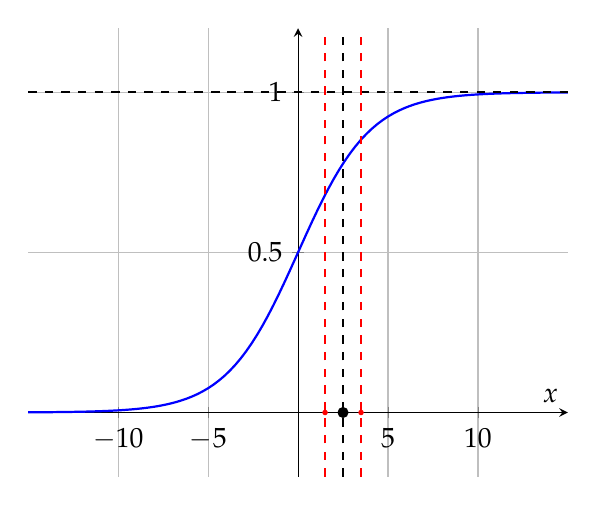
\begin{tikzpicture}
		\begin{axis}[
			axis lines=middle,
			xlabel=\(x\),
			yticklabel style={
				/pgf/number format/fixed,
				/pgf/number format/precision=1
			},
			ytick={0,0.5,1},
			xtick={-10,-5,0,5,10},
			grid,
			domain=-15:15,
			samples=100,
			ymax=1.2, % Adjusted y-axis to go a bit above 1
			ymin=-0.2
			]
			\addplot[blue,thick] {1/(1+exp(-0.5*x))};
			\addplot[dashed, black, thick] {1}; % Dashed horizontal line at y=1
			\fill [black] (axis cs:2.5,0) circle (2pt);
			\fill [red] (axis cs:1.5, 0) circle (1pt); 
			\fill [red] (axis cs:3.5, 0) circle (1pt); 
			\addplot[black, thin, dashed] coordinates {(2.5,-0.2) (2.5,1.2)};
			\addplot[red, thin, dashed] coordinates {(1.5,-0.2) (1.5,1.2)};
			\addplot[red, thin, dashed] coordinates {(3.5,-0.2) (3.5,1.2)};
		\end{axis}
	\end{tikzpicture}
	\caption{Example of sigmoid function TODO}
	\label{fig:sigmoid function}
\end{figure}

\usetikzlibrary{positioning}
\begin{tikzpicture}[node distance=1.5cm]
	% Nodes
	\node[circle, draw] (A) {A};
	\node[circle, draw, right=of A] (B) {B};
	\node[circle, draw, right=of B] (C) {C};
	\node[circle, draw, below=of A] (D) {D};
	\node[circle, draw, below=of B] (E) {E};
	\node[circle, draw, below=of C] (F) {F};
	
	% Edges
	\draw (A) -- (B);
	\draw (B) -- (C);
	\draw (A) -- (D);
	\draw (B) -- (E);
	\draw (C) -- (F);
	\draw (D) -- (E);
	\draw (E) -- (F);
\end{tikzpicture}
	
	\subsection{Emission probabilities}\label{subsec:emission probabilities}
	
	We consider several different types of data to inform about $\x$. This data may be of different dimensionality, e.g. may only discriminate along a subset of the axes or at a higher scale along some axes. For a particular data set $d=1, \ldots, D$, let $\bxi_d=\{\xi_{d1}, \ldots, \xi_{du}\}$ denote the sets of distinguished compartments. We then define the presence of ($\x(\xi_{du})=1$) or absence ($\x(\xi_{du})=0$) in set $\xi_{du}, u=1\ldots,U,$ as
	
	\begin{equation}
		\x(\xi_{du}) = \min \left(1, \sum_{c \in \xi_{du}} x_c \right).
	\end{equation}

	\subsection{Data sources}\label{subsec: data sources}
	We consider two sets of data informative about $\x$: i) Presence-absence data obtained with mass-spectrometry and ii) presence-only reports of specific metabolites in specific species.
	
	\subsubsection{Mass spectrometry}
	 Let $\bd _{sj}=(d_{sj1}, \ldots, d_{sjM})$ be the presence-absence vector of each metabolite $m$ obtained with mass-spectrometry run $j=1,\ldots,J_s$ performed on species $s$. Assuming a false-positive and false-negative error rates $\epsilon_{01}$ and $\epsilon_{10}$, respectively, we have
	
	\begin{equation}
		\P(\bd_{sj}|\x, \epsilon_{01}, \epsilon_{10}) = \prod_m \left[ x_{sm}\left(\epsilon_{10}^{1-d_{sjm}}(1-\epsilon_{10})^{d_{sjm}}\right) + (1-x_{sm})\left( \epsilon_{01}^{d_{sjm}}(1-\epsilon_{01})^{1-d_{sjm}}\right)\right]
	\end{equation}
	\subsubsection{LOTUS}
	
	As previously stated, LOTUS database \cite{rutzLOTUSInitiativeOpen2022} lists known occurrences of metabolites in species. Let $L_{ms} = 1$ denote a known occurrence of metabolite $m$ in species $s$, while $L_{ms}=0$ denotes that no evidence for such an occurrence has been reported, either because the metabolite $m$ is truly absent in species $s$ or because of a lack of research effort.
	
	Let us denote by $R_{sm}$ the probability of discovery of metabolite $m$ in species $s$ such that
	\begin{equation}\label{eq:prob lotus given x and Rsm}
		\P(L_{ms}|\x(\xi(m,s)), R_{ms}) = 
		\begin{cases}
			0 \quad &\mathrm{if\ } \x(\xi(m,s))=0 \mathrm{\ and\ } L_{ms} = 1,\\
			1 \quad &\mathrm{if\ } \x(\xi(m,s))=0 \mathrm{\ and\ } L_{ms} = 0,\\
			R_{ms} \quad &\mathrm{if\ } \x(\xi(m,s))=1 \mathrm{\ and\ } L_{ms} = 1,\\
			1- R_{ms} \quad &\mathrm{if\ } \x(\xi(m,s))=1 \mathrm{\ and\ } L_{ms} = 0,
		\end{cases}
	\end{equation}
	
	where $\xi(m,s)$ is the set of compartments relevant for metabolite $m$ and species $s$, i.e. all compartments $c$ for which $\tau_\M(c)=m$ and $\tau_\S(c)=s$.
	
	To quantify the research effort $R_{ms}$ of a particular entry $L_{ms}$, we will rely on two measures, the total number of relevant papers published for metabolite $m$ ($P_m$) and for species $s$ ($Q_s$), such that
	
	\begin{equation}\label{eq:research effort}
		R_{ms} = 1 - e^{-\gamma P_m - \delta Q_s}
	\end{equation}
	with positives scalars $\gamma$ and $\delta$. In \Cref{fig:DAG naive model} we show a  Directed Acyclic Graph (DAG) of the proposed model. 


	\begin{figure}
	\centering
	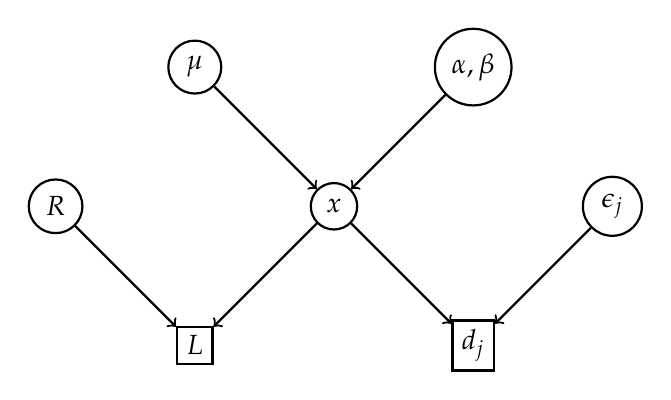
\begin{tikzpicture}[node distance={25mm}, thick, main/.style = {draw, circle}]
			\node[main] (1) {$\boldmath{x}$};
			\node[main] (2) [above left of=1] {$\mu$};
			\node[main] (3) [above right of=1] {$\alpha, \beta$};
			\node[draw] (4) [below right of=1] {$d_{j}$};
			\node[draw] (5) [below left of=1] {$L$};
			\node[main] (6) [above right of=4] {$\epsilon_j$};
			\node[main] (7) [above left of=5] {$R$};
	
			\draw[->] (2) -- (1);
			\draw[->] (3) -- (1);
			\draw[->] (1) -- (4);
			\draw[->] (1) -- (5);
			\draw[->] (6) -- (4);
			\draw[->] (7) -- (5);
		\end{tikzpicture}
	\caption{DAG of the \textit{naive model}. $x$ represents the presence/absence of a molecule in a specific species. With $\mu$ the average presence along a specific axis, $\alpha$ and $\beta$ an axis specific intercept and a positive scalar respectively. $R$ represents the research effort given for $x$, $L$ is the occurrence of $x$ in the LOTUS database and $\epsilon_j$ the $j^{th}$ mass spectrometry run for a specific species. }
	\label{fig:DAG naive model}
	\end{figure}

\section{Random Markov Field}\label{sec:methods:random markov field}

As previously stated, our objective is to infer the occurrence or absence of metabolites across a collection of samples, which are differentiated by discrete dimensions such as species, tissue type, and environmental conditions or any other arbitrary dimension. We hypothesize that the distribution pattern of these metabolites is moderated by shared characteristics within each dimension. For instance, metabolites can exhibit a similar distribution across phylogenetically close species, or if their synthesis pathways are interrelated. To quantitatively represent such similarities, we use a Markov random field approach \cite{sherringtonSolvableModelSpinGlass1975, kindermannMarkovRandomFields1980}.

Let $D$ denote the total number of dimensions. Without any loss of generality, we assume the first dimension corresponds to the metabolite. Each dimension, denoted by $d=1, \ldots, D$, consists of a set $\E_d$ of discrete entities (e.g., individual species along the species dimension). We model similarities between entries of dimension $d$ using a Markov process along a known tree $\T_d$ consisting of $\N_d = \E_d \cup \R_d \cup \I_d$ nodes, of which the entries $\E_d$ are leaves, connected to the set of roots $\R_d$ through a set $\I_d$ of internal nodes. We thus have $\E_d \cap \R_d = \varnothing$, $\E_d \cap \I_d = \varnothing$ and $\R_d \cap \I_d = \varnothing$. For every node $n \in \N_d, n \notin \R_d$ that is not a root, we denote $p(n) \in \N_d$ its parent node and $b(n) \geq 0$ the length of the branch connecting it to its parent.

We denote $\X$ a Markov Random Field of which each variable $x \in \X$ represents a unique combination of nodes from each dimension $D$, indicating the presence ($x=1$) or absence ($x=0$) of a metabolite. Let $\delta_d(x) \in \N_d$ reflect the node of $x$ in dimension $d$ with $\delta_1(x)$ indicating the metabolite of $x$, and let $\delta(x)=(\delta_1(x), \ldots, \delta_D(x))$. We only consider two sets of variables: 1) the set $\Y$ of variables representing an entry in each dimension such that for a variable $y\in\Y$, $\delta_d(y) \in \E_d$ for all $d=1, \ldots, D$, and 2) the set $\Z$ of variables representing leaves in all dimensions except one such that for a variable $z \in \Z$, $\delta_k(z) \in \I_k$ and $\delta_d(z) \in \E_d$ for all $d \neq k$. We then have $\X = \Y \cup \Z$ and $\Y \cap \Z = \varnothing$.

We suppose that the joint density of $\X$ can be factorized over a set of cliques $\Ccal$. Each clique $c \in \Ccal$ consist of a set of variables $x_1, x_2, \ldots \in \X$ that represent the same leaves in all but one dimension $k$. Specifically, for all $x \in c$, $\delta_d(x) \in \E_d$ for all $d \neq k$ and $\delta_k(x) \in \N_k$, and for all $x_i, x_j \in c$, $\delta_{-k}(x_i) = \delta_{-k}(x_j)$, where $\delta_{-k}(x)$ denotes the vector of nodes of $x$ in all dimensions but $k$. For such a clique, we will refer to the dimension $\nu(c) = k$ as its \emph{variable} dimension and will denote by $\delta_{-\nu(c)}(c)$ the vector of nodes in the \emph{fixed} dimensions. By definition, $\delta_{-\nu(c)}(c)=\delta_{-\nu(c)}(x)$ for every $x \in c$.

We will further denote by $\Ccal_k \subset \Ccal$ the subset of cliques that share the variable dimension $k$, i.e. $\nu(c)=k$ for all $c \in \Ccal_k$. Note that each clique is in exactly one subset ($\Ccal_k \cap \Ccal_d = \varnothing$ for all $k \neq d$) and cliques of the same subset do not share any variables ($c_1 \cap c_2 = \varnothing$ for all $c_1, c_2 \in C_k$). However, each variable $x \in \Y$ will be part of exactly one clique from each subset: the clique $c \in \Ccal_k$ for which $\delta_{-k}(c) = \delta_{-k}(x)$. In contrast, each variable $x \in \Z$ will be part of exactly one clique: the clique $c \in \Ccal$ for which $\delta_{-\nu(c)}(c) = \delta_{-\nu(c)}(x)$ and $\delta_{\nu(c)}(x) \in \I_{\nu(c)}$.

The joint density of $\X$ factorizes as
\begin{equation}
	\P(\X) = \prod_{d=1}^D \prod_{c \in \Ccal_d} \phi(c),
\end{equation}

where
we model the clique functions $\phi(c)$ using a Markov model along tree $\T_d$. Let

\begin{equation}
	\bLambda_c =
	\begin{pmatrix}
		-\mu_{c1} & \mu_{c1}\\
		\mu_{c0} & -\mu_{c0}\\
	\end{pmatrix}
\end{equation}

be the rate matrix for changes between states 0 and 1 along the tree. For each node $n \in \N_d, n \notin \R_d$ that is not a root, the transition probabilities between parent node $p(n)$ and $n$ are then given by

\begin{equation}
	\bP(n) = \exp(\bLambda_c b(n)).
\end{equation}

We assume the root state probabilities are given by the stationary distribution of the Markov chain:
\begin{equation}
	\bP_{\infty} = \left(\frac{\mu_{c0}}{\mu_{c0} + \mu_{c1}}, \frac{\mu_{c1}}{\mu_{c0} + \mu_{c1}}\right).
\end{equation}


The clique function $\phi(c)$
\begin{equation}
	\phi(c) = \prod_{x \in c, }\Big( \Ind(x \in \R_{\nu(c)})[\bP_{\infty}]_x + \Ind(x \notin \R_{\nu(c)}) [\bP(\delta_{\nu(c)}(x))]_{p_{c}(x), x} \Big)
\end{equation}

where we used the shorthand $x \in \R_{\nu(c)}$ for $\delta_{\nu(c)}(x) \in \R_{\nu(c)}$ to indicate whether the node in the variable dimension of $c$ of $x$ is a root and $p_{c}(x)$ to identify the variable $z \in c$ for which $\delta_{\nu(c)}(z) = p(\delta_{\nu(c)}(x))$.

\begin{figure}[h]
	\centering
	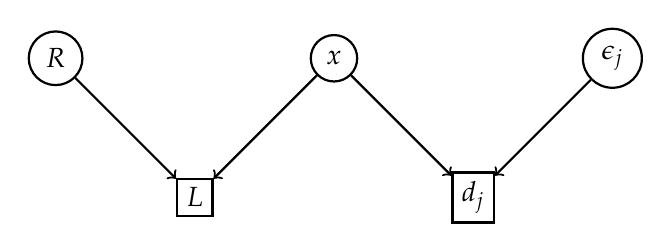
\begin{tikzpicture}[node distance={25mm}, thick, main/.style = {draw, circle}]
		\node[main] (1) {$\boldmath{x}$};
		\node[draw] (4) [below right of=1] {$d_{j}$};
		\node[draw] (5) [below left of=1] {$L$};
		\node[main] (6) [above right of=4] {$\epsilon_j$};
		\node[main] (7) [above left of=5] {$R$};
		
		\draw[->] (1) -- (4);
		\draw[->] (1) -- (5);
		\draw[->] (6) -- (4);
		\draw[->] (7) -- (5);
	\end{tikzpicture}
	\caption{DAG for the RMF model. $x$ represents the presence/absence of a molecule in a specific species. $R$ represents the research effort given for $x$, $L$ is the occurrence of $x$ in the LOTUS database and $\epsilon_j$ the $j^{th}$ mass spectrometry run for a specific species.}
	\label{fig:DAG_model}
\end{figure}

In \Cref{fig:DAG_model}, we illustrate a possible Directed Acyclic Graph (DAG) representation of the proposed model.

\subsection{Data sources}
The probabilities of the data given $x$ were formulated employing the same model as delineated in \Cref{subsec: data sources}.

\section{Graph Convolution Neural Network (GraphSAGE)}\label{sec:theory:HinSAGE}
The low-dimensional representation of nodes within large graphs plays a critical role in various domains of scientific research and industrial applications, such as bioinformatics, social networks, and content recommendation systems. The utilization of these embeddings has proven effective in diverse prediction tasks, including clustering, node classification, and link prediction. However, traditional methods for generating these embeddings have predominantly focused on the transductive setting, requiring all nodes to be present during training and thus limiting generalization to unseen nodes or entirely new subgraphs \cite{groverNode2vecScalableFeature2016, perozziDeepWalkOnlineLearning2014}.

GraphSAGE (SAmple and aggreGatE) \cite{hamiltonInductiveRepresentationLearning2017} was presented as a solution to this challenge, offering a general inductive framework that leverages both node feature information and topological structure. Unlike transductive approaches, which rely on matrix factorization and are constrained to fixed graphs, GraphSAGE is designed to efficiently generate embeddings for previously unseen nodes.

The novelty of GraphSAGE lies in its ability to learn a function that generates embeddings through the sampling and aggregation of features from a node's local neighbourhood. It utilizes a set of trainable aggregator functions that encapsulate information from different search depths (hops), or away from a given node. By simultaneously learning the topological structure and distribution of node features in the neighbourhood, GraphSAGE accommodates feature-rich graphs as well as graphs lacking specific node features.

The applicability of GraphSAGE extends beyond simple convolutions, embracing a framework that generalizes Graph Convolutional Networks (GCNs) for the task of inductive unsupervised learning \cite{kipfSemiSupervisedClassificationGraph2016}. Unlike traditional methods that optimize embeddings for each node, GraphSAGE's inductive approach promotes efficiency and adaptability, allowing for a seamless alignment of newly observed subgraphs with pre-existing node embeddings.

GraphSAGE is particularly well-suited for the task of predicting which molecule is present in which species due to its robust inductive learning framework that generalizes to unseen nodes and subgraphs. In the context of biological data, such as molecular structures and species interactions, GraphSAGE's ability to leverage both the topological structure and node feature information offers a powerful means to understand the complex relationships within and across molecular graphs. Its novel approach of sampling and aggregating features from a node's local neighbourhood enables the capture of intricate patterns and structural properties that can be essential in identifying molecular presence across species. Furthermore, the inductive nature of GraphSAGE allows for the efficient generalization across different organisms, facilitating the prediction in entirely new or evolving graphs.

HinSAGE, a derivative of GraphSAGE, has been specifically designed to handle heterogeneous graphs, where nodes and edges can be of various types. Developed by CSIRO's Data61, HinSAGE adeptly extends the foundational principles of GraphSAGE to contexts where the graph's heterogeneity introduces additional complexities. Unlike homogeneous graphs where the relation between nodes is more uniform, heterogeneous graphs present varying relationships and patterns, which HinSAGE is explicitly tailored to capture. By learning distinct embeddings for different types of nodes and relations, HinSAGE can uncover nuanced relationships within complex networks. This makes HinSAGE especially valuable for tasks such as predicting links within a bipartite graph, where one set of nodes represents species and another molecules. HinSAGE's capability to seamlessly navigate the intricacies of such heterogeneous structures ensures a richer and more accurate representation of the connections, fostering improved predictive accuracy for link prediction tasks in biological contexts where species-molecule interactions need to be discerned.

\chapter{Methods}\label{chap:Methods}
\section{Naive model}
Prior to the application of actual experimental data, a series of simulations were executed to evaluate the feasibility of estimating the entire set of parameters from the information contained within our dataset. Specifically, the variable $\mu$ was generated by sampling from a normal distribution with mean value of $0$ and variance of $1$. Meanwhile, the parameters $\alpha$, $\beta$, $\gamma$, and $\delta$ were each modelled using distinct exponential distributions, where individual values for the rate parameter $\lambda$ were attributed to each. In order to replicate the observed phenomenon, the number of papers per species $Q_s$ and per molecule $P_m$, were synthetically constructed by drawing from a Poisson distribution. Additionally, the variable $\sigma$ was simulated by drawing from a Wishart distribution \cite{wishartGENERALISEDPRODUCTMOMENT1928}.

As elaborated in \Cref{sec:methods:Naive approach}, the simulation process was initiated by drawing probabilities that $x=1$ from the \textit{expit} function, as defined in \Cref{eq:logit of X}. 
To emulate this binary characteristic, samples were subsequently drawn from a Bernoulli distribution, where the probability parameter was informed by the previous \textit{expit} function. Building upon this stochastic framework, the probabilities of LOTUS were constructed in accordance with \Cref{eq:prob lotus given x and Rsm,eq:research effort}. A  condition was imposed such that if $x$ for any given pair was $0$, then the corresponding probability was explicitly set to $0$.

These tailored probabilities were then employed as parameters for another Bernoulli distribution, generating binary outcomes that determined the number of papers associated with each pair. Specifically, if the result was $0$, the number of papers for that particular pair was set to $0$. Conversely, if the result was $1$, the number of papers for that pair was assigned based on random Poisson values that had been drawn previously in the simulation process.

This systematic approach resulted in the production of a simulated $x$ and a corresponding simulated LOTUS. This led to the occurrence of certain pairs that appearing empty, even though the molecule was indeed present within the species.

%These simulations were performed using numpy v1.23.5 \cite{harrisArrayProgrammingNumPy2020}, scipy v1.10.0 \cite{virtanenSciPyFundamentalAlgorithms2020} and numba v0.56.4 \cite{lam2015numba}. 
All codes are available on \href{https://github.com/commons-research/anticipated-lotus}{GitHub}.
 
\section{Random Markov Field}
Due to time constraints of the thesis, test and simulation for this model were not performed. Code is available both on \href{https://bitbucket.org/wegmannlab/metabolite_inference/src/master/}{Bitbucket} and on \href{https://github.com/anticipated-lotus/metabolite_inference}{GitHub}.

\section{HinSAGE}\label{sec:methods:HinSAGE}
The LOTUS database was aggregated to include only unique pairs of molecules and species. Once aggregated, the data was randomly partitioned into two subsets: 70\% allocated for training and 30\% for testing, adhering to common practices in machine learning and data analysis.

Graphs were systematically constructed for both the training and testing subsets using the software library NetworkX v3.1 \cite{SciPyProceedings_11}. In these graphs, individual nodes were designated to represent each molecule and species. When a specific species-molecule pair was identified in the LOTUS database, a directed edge was drawn between the two corresponding nodes. This procedure led to the creation of a bipartite graph, with directed edges labeled as "has" from species to molecules and "present in" from molecules to species.

The species' features were defined by extracting their phylogenetic information through the GBIF API \cite{GBIF, GbifPygbif2023}. Molecules' features were composed of their classification data from Classyfire \cite{djoumboufeunangClassyFireAutomatedChemical2016} and their Morgan Fingerprint \cite{rogersExtendedConnectivityFingerprints2010}, encoded using a 128-bit representation and a radius of 2.

In the preprocessing stage, features corresponding to both species characteristics and molecules' Classyfire properties were transformed through binary encoding. This transformation was essential to represent these categorical attributes as numerical values, thus making them suitable as features for the nodes within the graph. In the case of the molecules, two different sets of features, namely the binary-encoded Classyfire attributes and the Morgan Fingerprint, were concatenated to form a unified feature vector.

The model training was carried out using the Stellargraph library \cite{StellarGraphMachineLearning2018}. Two distinct models were trained to handle different relationships within the graph; one was tailored to the edges labeled "has" and the other to the edges described as "present in".

The HinSAGE models were configured with two layers, comprising 1024 neurons in each layer. The first layer was designed with a neighborhood sampling size of 3, enabling the model to encapsulate the local structural information, while the second layer utilized a sampling size of 1, thus focusing on immediate neighbors. By employing this hierarchical structure, the models could capture different scales of locality in the graph.

Furthermore, the HinSAGE models were implemented with a mean aggregator function, which served to combine the features of the neighboring nodes, thus generating a representative feature vector for each target node. A dropout rate of 0.3 was applied to mitigate the risk of overfitting, and "elu" and "selu" activation functions were utilized in the respective layers. These activation functions were chosen for their properties in mitigating vanishing gradient problems, thereby aiding the convergence of the model during the training process.

All codes are available on \href{https://github.com/anticipated-lotus/GNN}{Github}.


\chapter{Results and Discussion}
\section{Naive approach}
In the preliminary stages of our research, we recognized the necessity to understand the behaviour of our model prior to applying it to the actual dataset. To achieve this, we carried out a series of simulations to assess if the model's parameters could be accurately estimated based on these synthetic data.

Specifically, we simulated 100 molecules and 10 species in alignment with the theoretical framework described by Equations \ref{eq:prob lotus given x and Rsm} and \ref{eq:research effort}.

For the parameter estimation process, we employed Markov Chain Monte Carlo (MCMC) techniques to accurately estimate the parameters $\gamma$ and $\delta$. The results of this estimation process were consistent and close to our simulated values, demonstrating the effectiveness of the approach.

Furthermore, we utilized Gibbs sampling as a specific tool within the MCMC framework to estimate the variable $x$. This method too yielded satisfactory results, corroborating the validity of our model in this aspect.

However, the challenges encountered during the modelling and simulation process were primarily centred around the convergence of the axis-specific intercepts $\mu$. This crucial component, detailed in Equation \ref{eq:logit of X}, resisted precise estimation through our initially chosen techniques. During this period of reevaluation, the proposition of interpreting our data as a graph surfaced, adding a new dimension to our perspective. Persisting with our original data treatment no longer seemed intuitive. Given the inherent structure and relationships in our dataset, transitioning to a graph-based approach felt more logical and natural. As a result, the inability to accurately estimate $\mu$ and the allure of a graph-centric methodology prompted us to explore alternative models and techniques, seeking a better alignment with the intrinsic characteristics of our data.

To reproduce our simulations, codes are available on \href{https://github.com/commons-research/anticipated-lotus}{GitHub}.

\section{Random Markov Field}
Due to time constraints of the thesis, test and simulation for this model were not performed.

However this could work since paper TODO $\ldots$

\section{HinSAGE}
After evaluating the models using unseen edge data, the performance metrics revealed differing accuracy levels for each model. Specifically, the model trained to predict the "present in" relationships exhibited an accuracy of 0.92. In contrast, the model aimed at predicting the "has" relationships demonstrated an accuracy of 0.8.

It is important to note that the threshold for determining the presence or absence of metabolites was set at a probability value of 0.5. Consequently, probabilities exceeding this threshold were categorized as a presence, denoted as $x=1$, whereas values below this threshold were classified as an absence, represented as $x=0$.










TODO We then decided to try to anticipate the entire LOTUS database i.e. get the probability of any combination of species-molecule pair. This resulted in a $\ldots$ 


Limitations: Sampling negatives edges is sampling only edges that do not exist yet. However this may lead to problems since by sampling negative edges, we might sample an edge that we may have but has not been discovered yet. 


%\section{Challenges: Data Sparsity and Detection Uncertainty}


\chapter{Applications and Implications}


\chapter{Conclusion and Future Work}
Question 1 : Do you want LOTUS anticipated ? 

Question 2 : Do you want the true presence/absence ?


Future work : Continue developing RMF. As shown in paper \cite{jiaGraphBeliefPropagation2021}, both model can work. 
\section{Knowledge Graph Completion}
Knowledge Graphs (KGs) provide a robust technique for the consolidation of diverse data and the modelling of complex interactions, crucial for areas like forecasting the natural products present in various species \cite{ehrlingerDefinitionKnowledgeGraphs2016}. 

In its simplest form, a graph is a data structure that designates items (or "nodes") and the links (or "edges") between them. In the context of our discussion, nodes might symbolize different species, while edges could denote a variety of relationships such as common ecosystems, shared characteristics, or the potential to yield similar natural products. Depending on the kind of the relationships, the graph can either be directed (representing asymmetric relations) or undirected (symbolizing symmetric relations).

Two primary categories of graphs exist: homogeneous and heterogeneous. A homogeneous graph possesses nodes and edges of the same category. In this scenario, a homogeneous graph might be comprised of species nodes interconnected by edges representing a particular connection, like a mutual ecosystem. Conversely, a heterogeneous graph contains nodes and edges of diverse types. For instance, a heterogeneous graph in this case could encompass nodes representing species, ecosystems, and natural products, linked through various relationships like "inhabits", "generates", or "has common traits with".

A specific kind of graph known as multigraphs permits multiple edges between the same pair of nodes and can also accommodate loops. This is advantageous when there are various types of relations between the same pair of nodes. Multigraphs are predominantly heterogeneous.

A Knowledge Graph (KG) is a distinct type of graph used to encode significant knowledge concerning a specific domain. It is a directed, heterogeneous multigraph with domain-specific semantics for its node and relation types. In this setting, a KG could be employed to encode knowledge about species and their capability to produce natural products. The nodes in the KG, also known as entities, could symbolize different species, ecosystems, or specific natural products. The directed edges, usually represented as triples (head, relation, tail), encapsulate the relationships between these entities.

Knowledge graph embeddings are techniques to convert the discrete entities and relations in a KG into continuous vectors in a high-dimensional space, while preserving the original relationships from the KG \cite{wangKnowledgeGraphEmbedding2017}. This conversion to a continuous vector space is especially valuable in predicting missing information, like forecasting a species' potential to produce a specific natural product based on its relations with other entities in the KG.

In conclusion, KGs and their corresponding embeddings act as an essential instrument for encoding and analysing multifaceted, relational data. Within the context of predicting natural products in species, they can encapsulate and represent complex relationships between species, ecosystems, and the natural products themselves, potentially contributing to the discovery and comprehension of new natural products.

%----------------------------------------------------------------------------------------
%	THESIS CONTENT - APPENDICES
%----------------------------------------------------------------------------------------

\appendix % Cue to tell LaTeX that the following "chapters" are Appendices

% Include the appendices of the thesis as separate files from the Appendices folder
% Uncomment the lines as you write the Appendices

%\include{Appendices/AppendixA}
%\include{Appendices/AppendixB}
%\include{Appendices/AppendixC}

%----------------------------------------------------------------------------------------
%	BIBLIOGRAPHY
%----------------------------------------------------------------------------------------
%\printbibliography
\renewcommand{\bibname}{References}
\bibliographystyle{unsrturl}
\bibliography{/Users/Marco/BibTex/MyBibTex}


%----------------------------------------------------------------------------------------

\end{document}  
